\section{History}\label{sec:history}

Three lines of work meet in this paper, and a fourth, recent one supplies its motivation. Figure~\ref{fig:history} places them on one time axis and Table~\ref{tab:history} lists what each contributes to the argument.

\begin{figure*}[t]
\centering
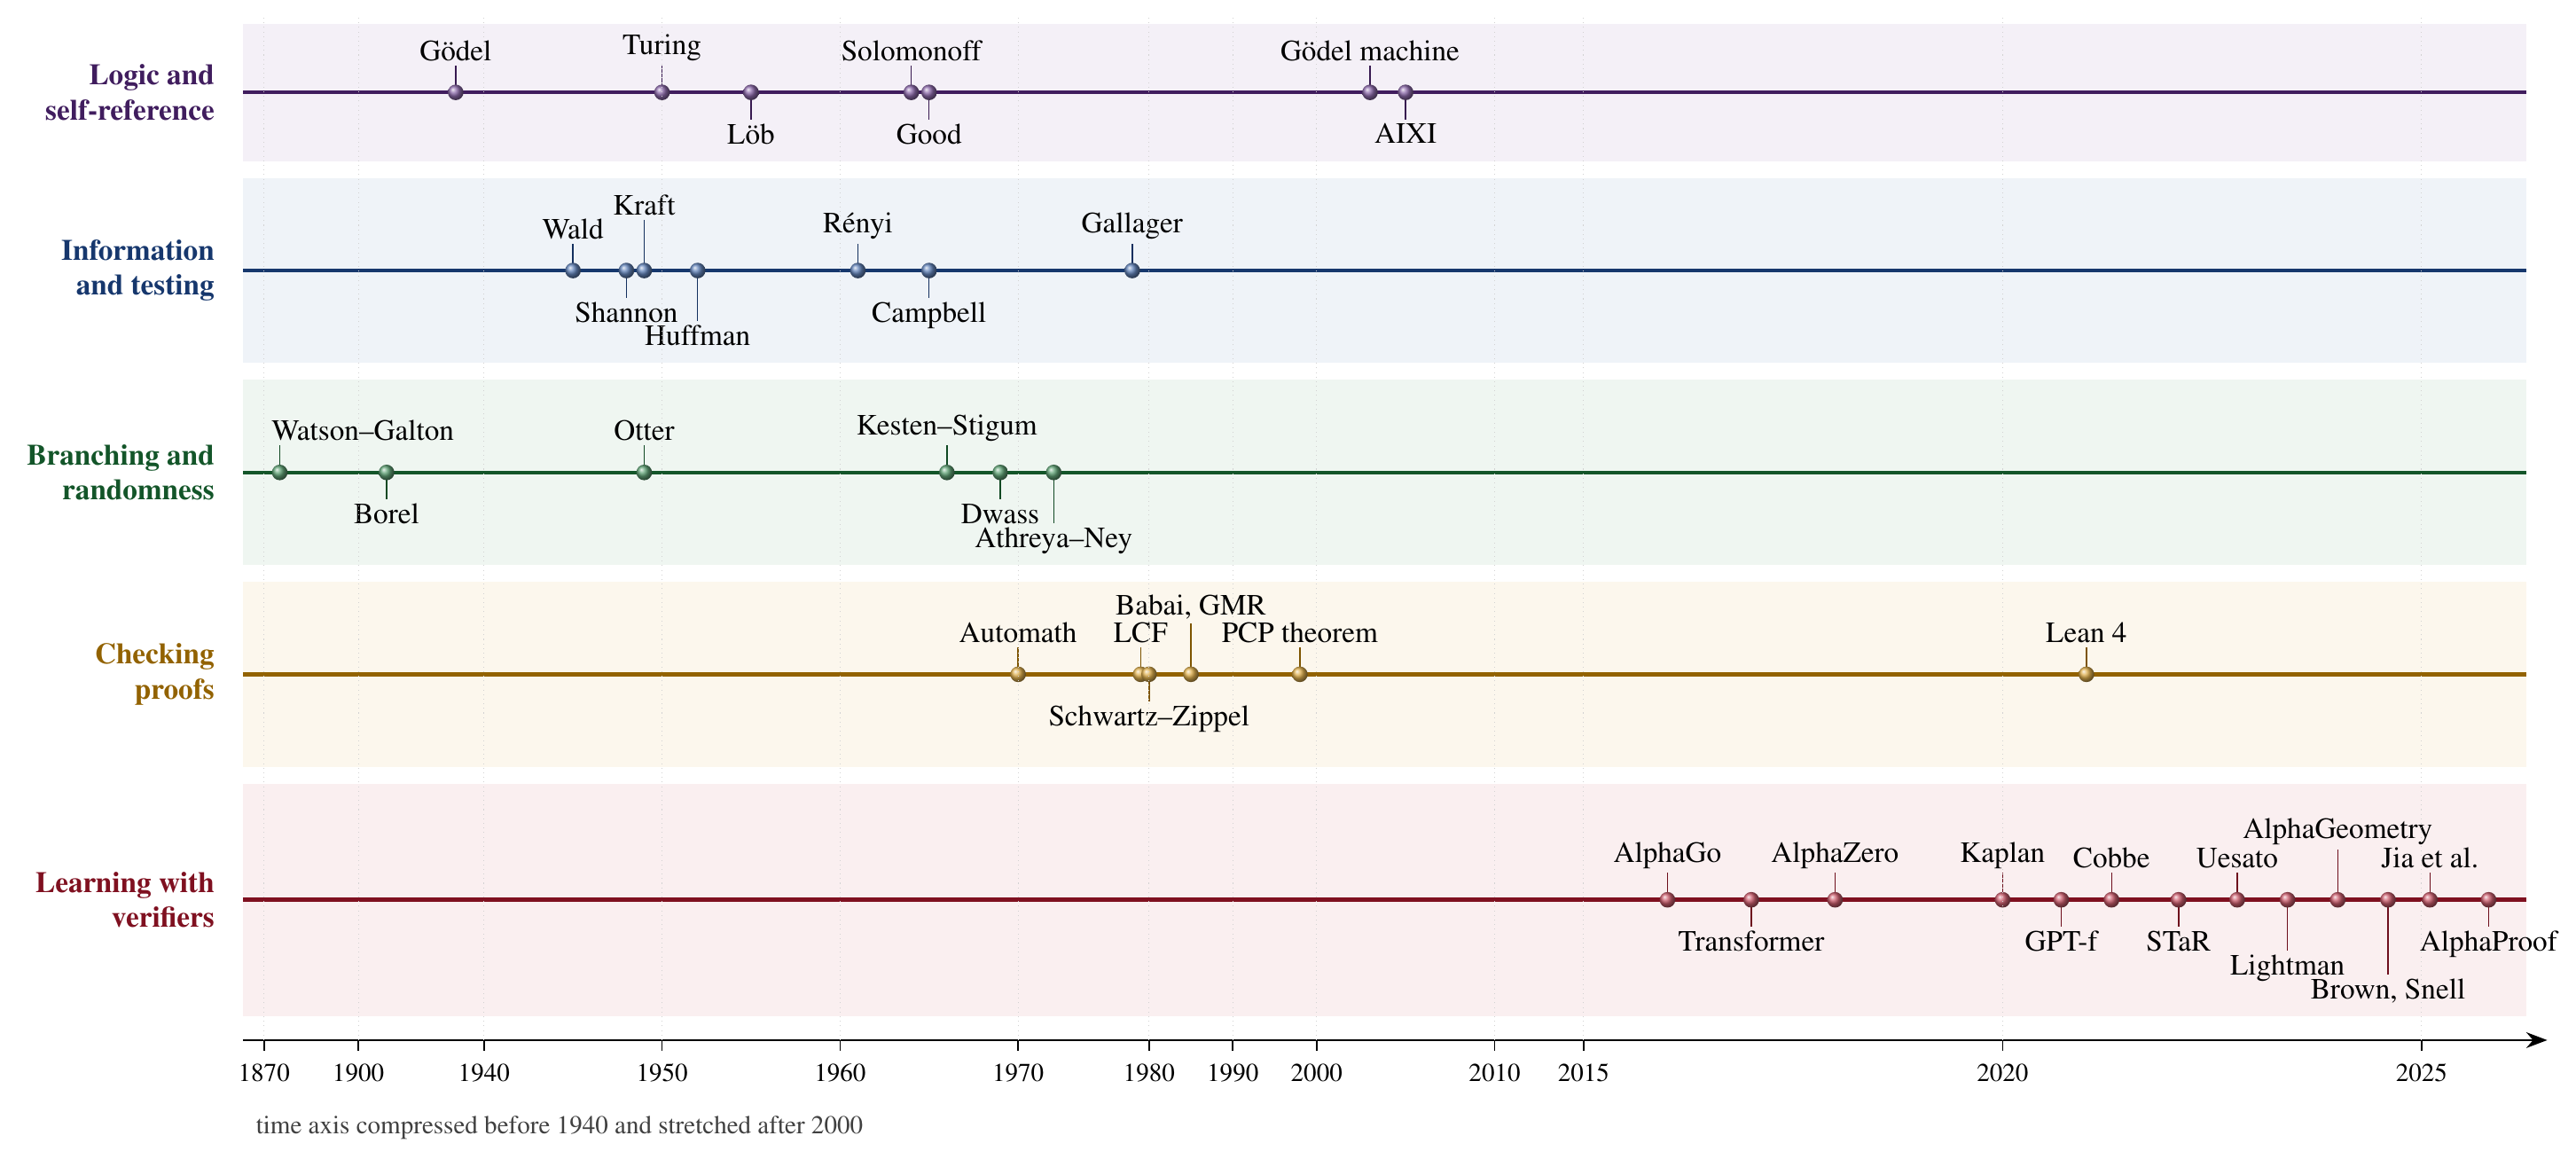
\includegraphics[width=\textwidth]{figures/fig_history}
\caption{Five lines of work on one time axis, with the scale stretched after 2015. Logic and self-reference: G\"odel's incompleteness theorems, Turing's learning machine, L\"ob's theorem, Solomonoff's induction, Good's intelligence explosion, the G\"odel machine and AIXI. Information and testing: Wald's sequential tests, Shannon's source coding, Kraft's inequality, Huffman's codes, R\'enyi's entropies, Campbell's coding theorem and Gallager's redundancy bound. Branching and randomness: the Watson--Galton problem, Borel's denumerable probabilities, Otter's multiplicative process, the Kesten--Stigum theorem, Dwass's total progeny and the monograph of Athreya and Ney. Checking proofs: Automath, LCF, the polynomial identity test of Schwartz and Zippel, interactive proofs, the PCP theorem and Lean~4. Learning with verifiers: from AlphaGo and the transformer to trained verifiers, process supervision, repeated sampling and AlphaProof.}
\label{fig:history}
\end{figure*}

\subsection{Self-reference and the intelligence explosion}

Turing's paper of 1950 already contains the idea of a machine that improves itself: rather than program an adult mind, one should program a child machine and educate it, and he expected the educated machine to be modified by its own experience \cite{Tur50}. Fifteen years later Good drew the consequence for machines better than their designers \cite{Goo66}. The formal theory of such machines met an obstacle at once, and the obstacle is logical. G\"odel's second incompleteness theorem shows that a consistent system containing arithmetic does not prove its own consistency \cite{God31}, and L\"ob's theorem sharpens it: if such a system proves that provability of a sentence implies the sentence, then it proves the sentence \cite{Lob55}.\footnote{L\"ob's theorem answers a question of Henkin. Let $T$ be a consistent recursively axiomatised extension of Peano arithmetic and $\mathrm{Prov}_{T}$ its provability predicate. If $T\vdash\mathrm{Prov}_{T}(\ulcorner\varphi\urcorner)\to\varphi$ then $T\vdash\varphi$. Applied to a self-modifying agent that keeps a successor only when it proves the successor sound, the theorem forbids the agent from accepting, in general, a successor that uses the same proof system with the same trust, since that acceptance would require the agent to prove a reflection principle for its own system. The present paper avoids the obstacle by replacing proofs of soundness with randomized checks of bounded error, whose reliability is a probability, not a theorem of the system.} An agent that rewrites itself only after proving that the rewrite is sound cannot in general accept a successor as strong as itself. Schmidhuber's G\"odel machine makes this precise in the other direction: it rewrites any part of its own code once it has found a proof that the rewrite increases expected utility, and is optimal among such strategies relative to its axioms \cite{Sch03}. Solomonoff's theory of inductive inference \cite{Sol64} and Hutter's AIXI \cite{Hut05} give the ideal, uncomputable agents against which the practical ones are measured.

The present paper does not ask for proofs. It asks for checks with a stated probability of error and counts what they cost. That shift, from certainty to bounded error, is the one complexity theory made between the 1970s and the 1990s.

\subsection{Coding and testing}

Shannon's theorem of 1948 says that a source with distribution $p$ cannot be encoded by a uniquely decodable code in fewer than $H(p)$ symbols on average, and that $H(p)+1$ can be reached \cite{Sha48}. Kraft's inequality, from his master's thesis of 1949, characterises the lengths of prefix codes \cite{Kra49}; McMillan extended it to all uniquely decodable codes \cite{McM56}; Huffman's algorithm of 1952 finds an optimal code \cite{Huf52}; Gallager bounded its redundancy \cite{Gal78}. R\'enyi introduced in 1961 a family of entropies $H_{\alpha}$ that share the additivity of Shannon's \cite{Ren61}, and Campbell showed in 1965 that $H_{\alpha}$ is the optimal mean length when long codewords are penalised exponentially \cite{Cam65}. The standard account is \cite{CT06}.

The connection with checking is older than it looks. Wald's sequential tests of 1945 already treat the trade-off between the number of observations and the two probabilities of error \cite{Wal45}, and Chernoff's exponent of 1952 \cite{Che52} and Hoeffding's inequality of 1963 \cite{Hoe63} give the rates at which repeated observations drive the error down. What seems not to have been noticed is that the optimal allocation of repetitions among many checks of unequal cost under a common error budget is a coding problem, with costs in the role of probabilities and repetitions in the role of codeword lengths. Theorems~\ref{thm:A} and~\ref{thm:C} make the identification exact.

\subsection{Branching and randomness}

The Watson--Galton paper of 1875 asked for the probability that a surname dies out, and reduced the question to the iteration of a generating function \cite{WG75}; the conclusion drawn there, that every family dies out, was wrong, and the correct criterion, extinction with probability one exactly when the mean number of sons is at most one, became standard only in the twentieth century. Otter's multiplicative process of 1949 put the theory in its modern form \cite{Ott49}, Kesten and Stigum proved in 1966 that the normalised population converges to a limit that is positive on survival exactly when $\EE\,\xi\log\xi<\infty$ \cite{KS66}, and Dwass related the total progeny to a random walk \cite{Dwa69}; the monograph of Athreya and Ney is the reference \cite{AN72}. Borel's paper of 1909 on denumerable probabilities contains the first form of the Borel--Cantelli lemma \cite{Bor09}, which decides here whether a sound singular chain keeps finitely many errors. Osgood's criterion of 1898 for blow-up of the equation $y'=f(y)$ \cite{Osg98} is the continuous form of the condition $\sum a_{n}<\infty$ for a singularity.

\subsection{Checking proofs}

De Bruijn's Automath \cite{dB70} and Milner's LCF \cite{GMW79} began the mechanical checking of proofs, and Lean~4 \cite{MU21} is the system used here. In parallel, complexity theory replaced certainty by bounded error. Schwartz and Zippel showed that a polynomial identity can be tested by evaluating at random points, with error at most the degree divided by the size of the field per run \cite{Sch80,Zip79}; Babai \cite{Bab85} and Goldwasser, Micali and Rackoff \cite{GMR89} introduced interactive proofs, in which a verifier is convinced with error probability that halves with each round; the PCP theorem showed that every proof can be written so that a verifier reads a constant number of its bits and errs with probability at most one half \cite{AS98,ALM98}. These are exactly the checks of the present paper: perfect completeness, soundness $\eps<1$ per run, and independent repetition.

\subsection{Learning with verifiers}

The fourth line is recent. AlphaGo \cite{SHM16} and AlphaZero \cite{SHS18} learned games by self-play against an exact referee, the rules of the game. Transformers \cite{VSP17} and the scaling of language models \cite{BMR20,KMH20,HBM22} produced generators of proofs and programs, and verifiers were added to them: Polu and Sutskever coupled a language model to the Metamath checker \cite{PS20}, Cobbe and coauthors trained verifiers to rank solutions of arithmetic problems \cite{CKB21}, Uesato and coauthors and Lightman and coauthors compared rewards for the final answer with rewards for every step \cite{UKK22,LKB23}, and chains of thought made the steps explicit \cite{WWS22}. Self-improvement loops followed: a model trained on its own checked rationales \cite{ZWM22}, on its own consistent answers \cite{HGH22}, on its own feedback \cite{MTG23} or on a constitution \cite{BKK22}. Spending computation at inference time, by sampling many candidates and keeping the checked ones, became a lever of its own \cite{BJE24,SLX24}. AlphaGeometry \cite{TWL24} and AlphaProof \cite{HMS25} reached olympiad level by searching against exact checkers. Errors of transformers on compositional tasks grow with the number of steps \cite{DLS23}, which is one reason to check every step.

The theory has followed. Jia, Rakhlin and Xie showed that learning from outcome supervision is statistically no harder than learning from process supervision, up to polynomial factors in the horizon \cite{JRX25}; Botta and coauthors showed that a process verifier can turn an intractable generation problem into a tractable one \cite{BLM25}; Rohatgi and coauthors showed that small errors of a learned verifier are amplified along a generation and designed a backtracking sampler that resists them \cite{RSS25}; Balcan and coauthors studied learned verifiers of chains of thought and the asymmetric role of their soundness errors \cite{BBF26}; Scrivens reported that classifier-based safety gates fail over many rounds of self-improvement while a verifier with analytic bounds does not \cite{Scr26}; Guo turned impossibility results into design rules \cite{Guo26}; Lu compared improvements of agentic systems through bounded verification and showed that independent majority amplification preserves the languages it defines \cite{Lu26}. On the growth side, Ord showed that singular growth requires the time around the feedback loop to tend to zero \cite{Ord26}, Anbar Jafari, Ozcinar and Anbarjafari gave testable conditions for runaway growth \cite{AOA25}, and the first author with Singha Roy and Samal studied phase transitions and predictability limits of general intelligence \cite{BSS26}. The verifier-gated engine of \cite{Bha26a} and the earlier analysis of the expulsion of a superintelligence from human control \cite{Bha21} are the two works of the first author on which the present architecture is built.

None of these works prices soundness. They bound sample complexity, query complexity, error amplification or growth rates, and they treat the verifier as given. The question here is how a fixed budget of false acceptances should be distributed over many checks of different costs, and what that distribution costs; the answer is an entropy, and it decides which singular takeoffs are sound.

\begin{table*}[t]
\caption{Milestones used in the paper. The last column says where each enters the argument.}
\label{tab:history}
\centering
\small
\begin{tabular}{@{}l l p{0.42\textwidth} l@{}}
\toprule
Year & Work & Contribution & Used in \\
\midrule
1875 & Watson, Galton \cite{WG75} & extinction of families by iterating a generating function & Theorem~\ref{thm:F} \\
1898 & Osgood \cite{Osg98} & blow-up of $y'=f(y)$ in finite time & Section~\ref{sec:scaling} \\
1909 & Borel \cite{Bor09} & denumerable probabilities, Borel--Cantelli & Theorem~\ref{thm:E} \\
1931, 1955 & G\"odel, L\"ob \cite{God31,Lob55} & limits of self-trust in formal systems & Section~\ref{sec:history} \\
1945 & Wald \cite{Wal45} & sequential tests and two probabilities of error & Section~\ref{ssec:twosided} \\
1948 & Shannon \cite{Sha48} & entropy as the optimal mean code length & Theorem~\ref{thm:A} \\
1949, 1956 & Kraft, McMillan \cite{Kra49,McM56} & lengths of prefix and decodable codes & Theorem~\ref{thm:C} \\
1949 & Otter \cite{Ott49} & multiplicative processes & Theorem~\ref{thm:F} \\
1952 & Huffman \cite{Huf52} & optimal prefix codes & Theorem~\ref{thm:C} \\
1952 & Chernoff \cite{Che52} & exponential rate of tests on sums & Proposition~\ref{prop:twosided} \\
1961, 1965 & R\'enyi, Campbell \cite{Ren61,Cam65} & entropies of order $\alpha$ and exponential code costs & Theorem~\ref{thm:D} \\
1965 & Good \cite{Goo66} & the intelligence explosion & Section~\ref{sec:intro} \\
1966 & Kesten, Stigum \cite{KS66} & the limit $Z_{k}/m^{k}$ on survival & Theorem~\ref{thm:F} \\
1979--1980 & Schwartz, Zippel \cite{Sch80,Zip79} & randomized identity tests with one-sided error & Section~\ref{sec:model} \\
1985--1998 & Babai; GMR; PCP \cite{Bab85,GMR89,AS98,ALM98} & bounded-error verification of proofs & Section~\ref{sec:model} \\
2003 & Schmidhuber \cite{Sch03} & self-rewriting after a proof of improvement & Section~\ref{sec:history} \\
2021--2023 & Cobbe; Uesato; Lightman \cite{CKB21,UKK22,LKB23} & trained verifiers, process and outcome rewards & Theorem~\ref{thm:gating} \\
2024--2025 & AlphaGeometry, AlphaProof \cite{TWL24,HMS25} & search against exact checkers & Section~\ref{sec:model} \\
2025--2026 & Jia et al.; Rohatgi et al.; Ord \cite{JRX25,RSS25,Ord26} & outcome supervision, verifier errors, singular growth & Sections~\ref{sec:chains}, \ref{sec:scaling} \\
\bottomrule
\end{tabular}
\end{table*}
